\documentclass{article}
\usepackage[utf8]{inputenc}
\usepackage{graphicx}
\usepackage{amsmath}
\usepackage{geometry}
\usepackage{listings}
\usepackage{xcolor}
\usepackage{float}

\geometry{a4paper, margin=1in}

\lstset{
    language=C,
    basicstyle=\ttfamily\small,
    keywordstyle=\color{blue},
    commentstyle=\color{green!60!black},
    stringstyle=\color{red},
    numbers=left,
    numberstyle=\tiny,
    numbersep=5pt,
    breaklines=true,
    showstringspaces=false,
    frame=single,
    tabsize=4
}

\title{HPC MPI TUTORIAL 19 REPORT}
\author{CS22B2015 -- HARSHITH B}
\date{\today}

\begin{document}

\maketitle

\section{Introduction}
This report analyzes the performance of parallel implementation for calculating the mean shift clustering algorithm using MPI. The execution time was measured for different numbers of MPI processes (1 to 6), and speedup was calculated to evaluate the scalability of the parallel implementation.

\section{Parallel Code Snippet}
The parallel implementation uses MPI to distribute the workload across multiple processes. Each process handles a portion of the data points, and the results are combined to produce the final clustering.

\section{Benchmark Results}
The benchmark was run with varying numbers of MPI processes, and the execution time was recorded for each configuration. All tests were performed with 15 centroids.

\begin{table}[H]
\centering
\begin{tabular}{|c|c|c|}
\hline
\textbf{MPI Processes} & \textbf{Time (seconds)} & \textbf{Num Centroids} \\
\hline
1 & 198.77 & 15 \\
2 & 101.22 & 15 \\
3 & 68.80 & 15 \\
4 & 51.56 & 15 \\
5 & 42.25 & 15 \\
6 & 35.78 & 15 \\
\hline
\end{tabular}
\caption{Execution time for different numbers of MPI processes}
\end{table}

\section{Performance Analysis}

\subsection{Execution Time vs Number of Processes}
Figure 1 shows the execution time as a function of the number of MPI processes. As expected, the execution time decreases as more processes are used, demonstrating the benefit of parallel processing.

\begin{figure}[H]
\centering
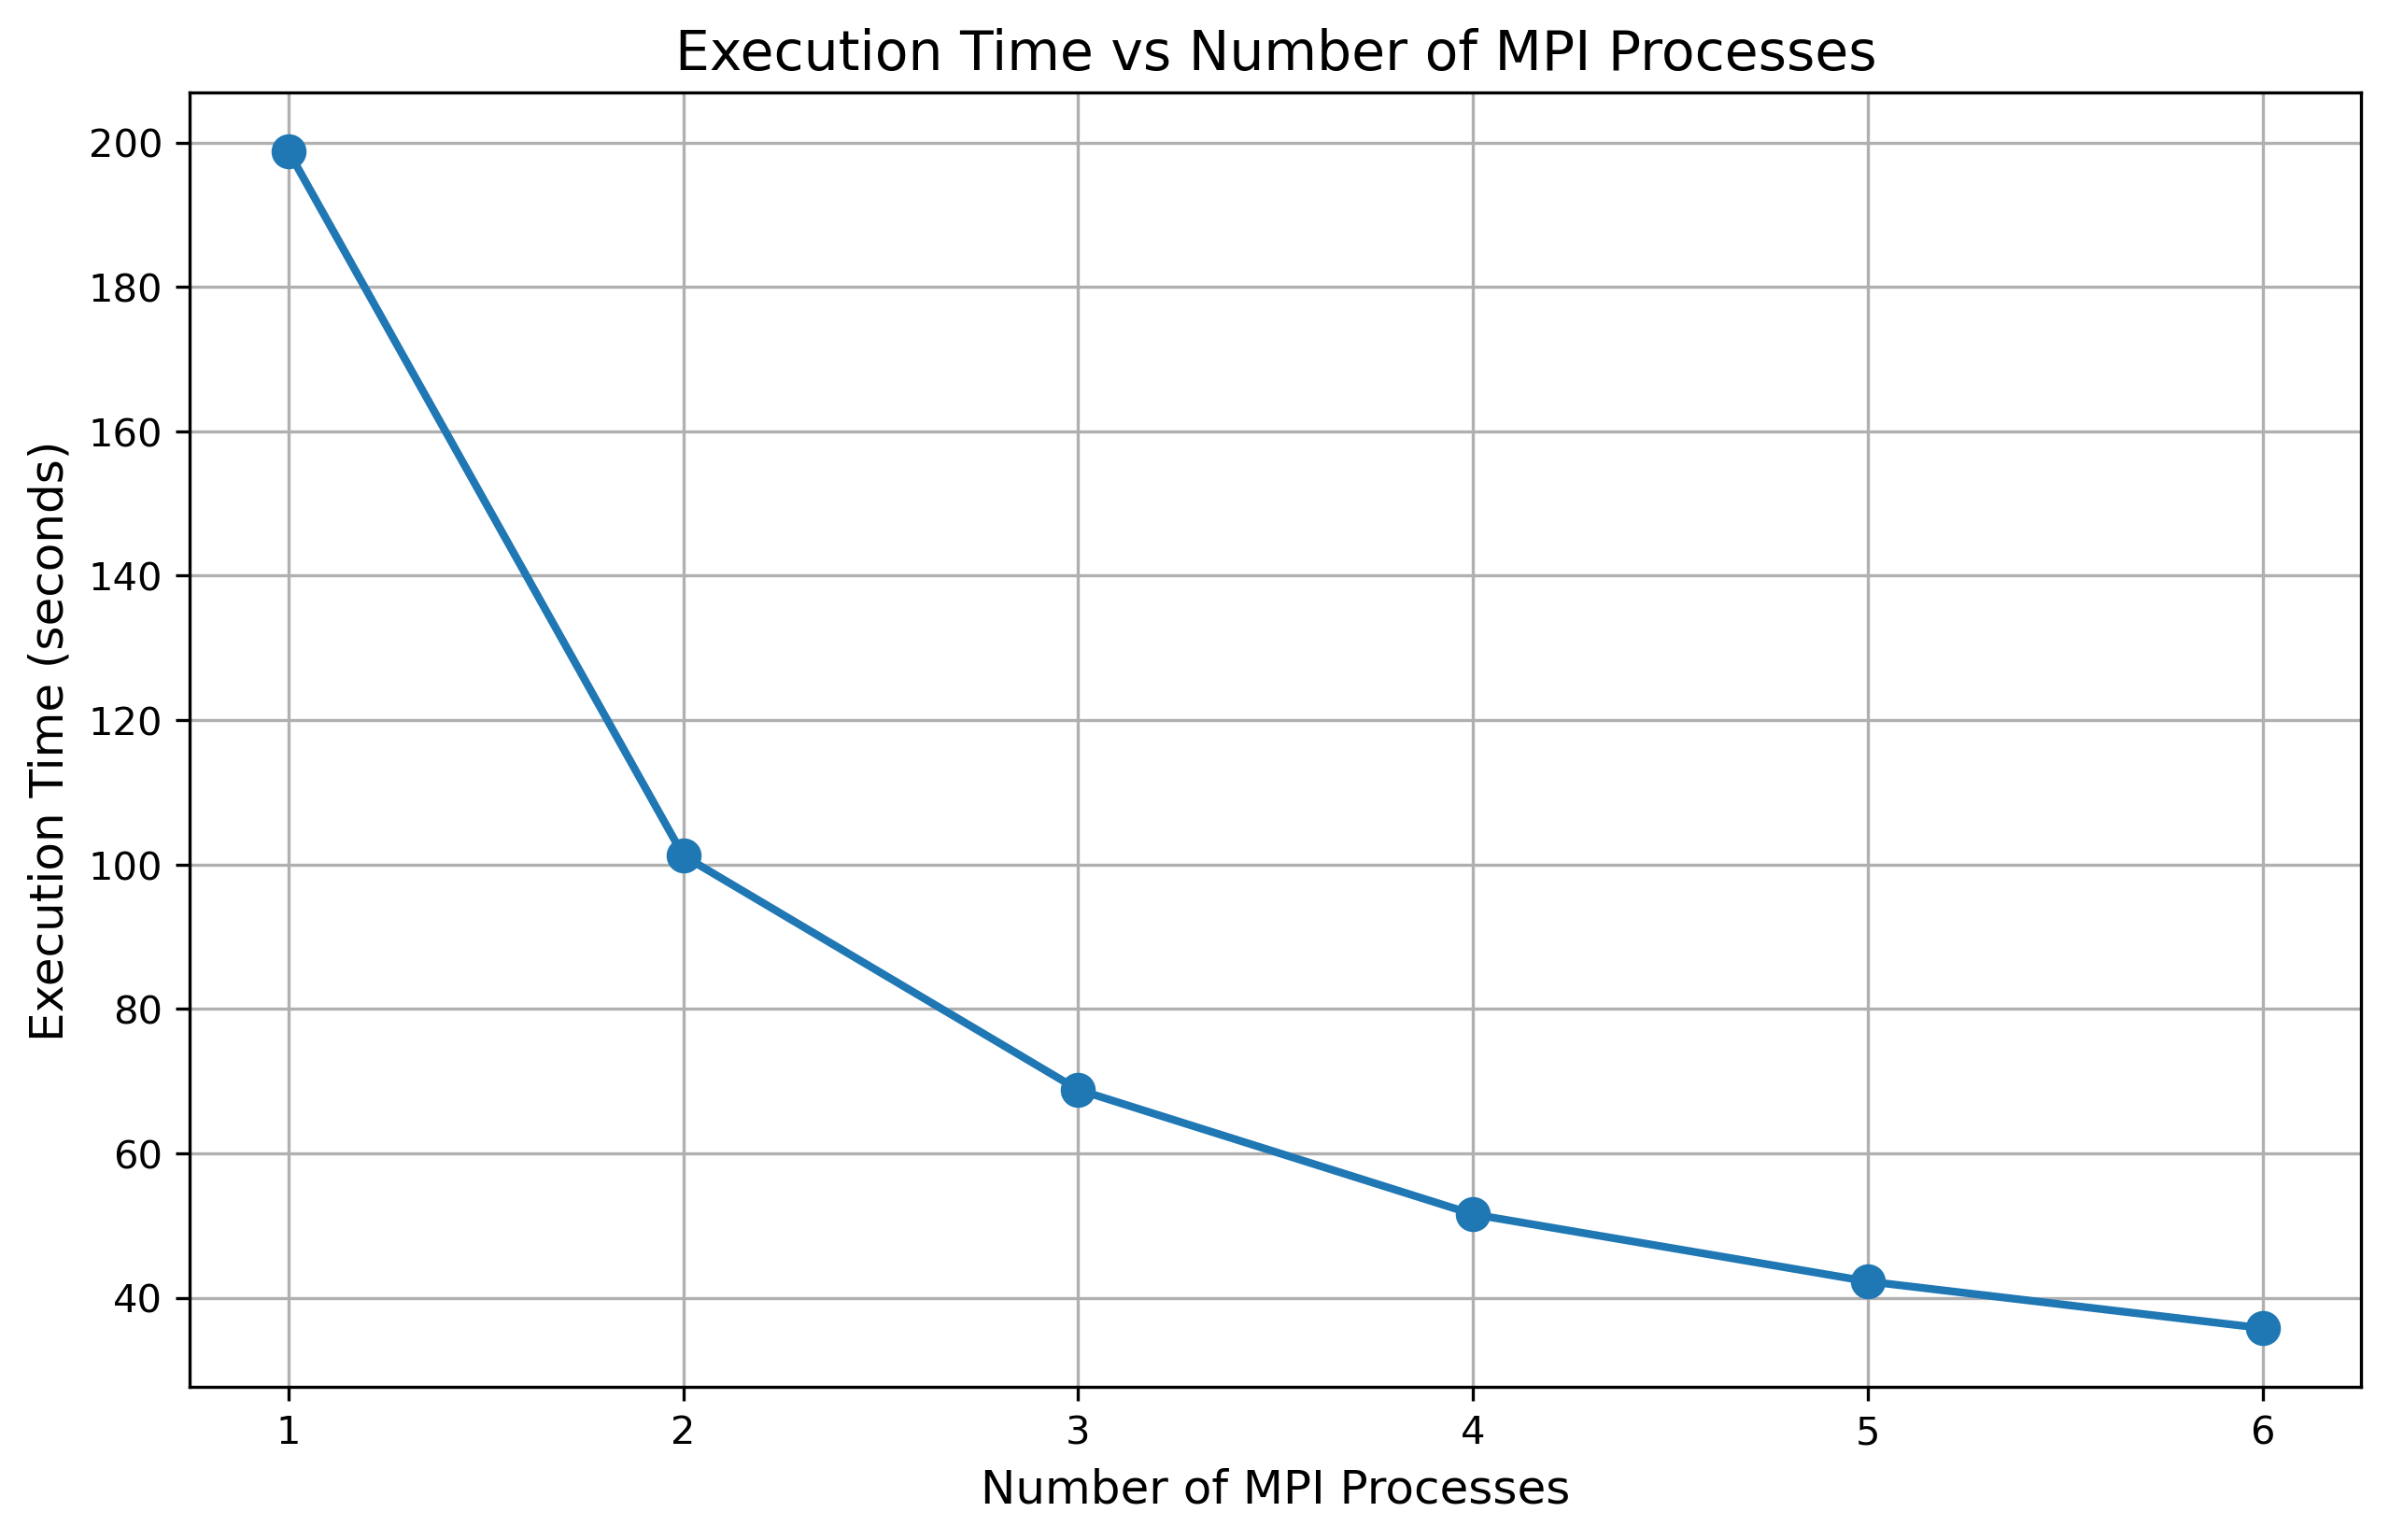
\includegraphics[width=0.8\textwidth]{time_vs_processes.png}
\caption{Execution Time vs Number of MPI Processes}
\end{figure}

\subsection{Speedup vs Number of Processes}
Figure 2 shows the speedup achieved with different numbers of MPI processes. The speedup is calculated as the ratio of the execution time with a single process to the execution time with multiple processes.

\begin{figure}[H]
\centering
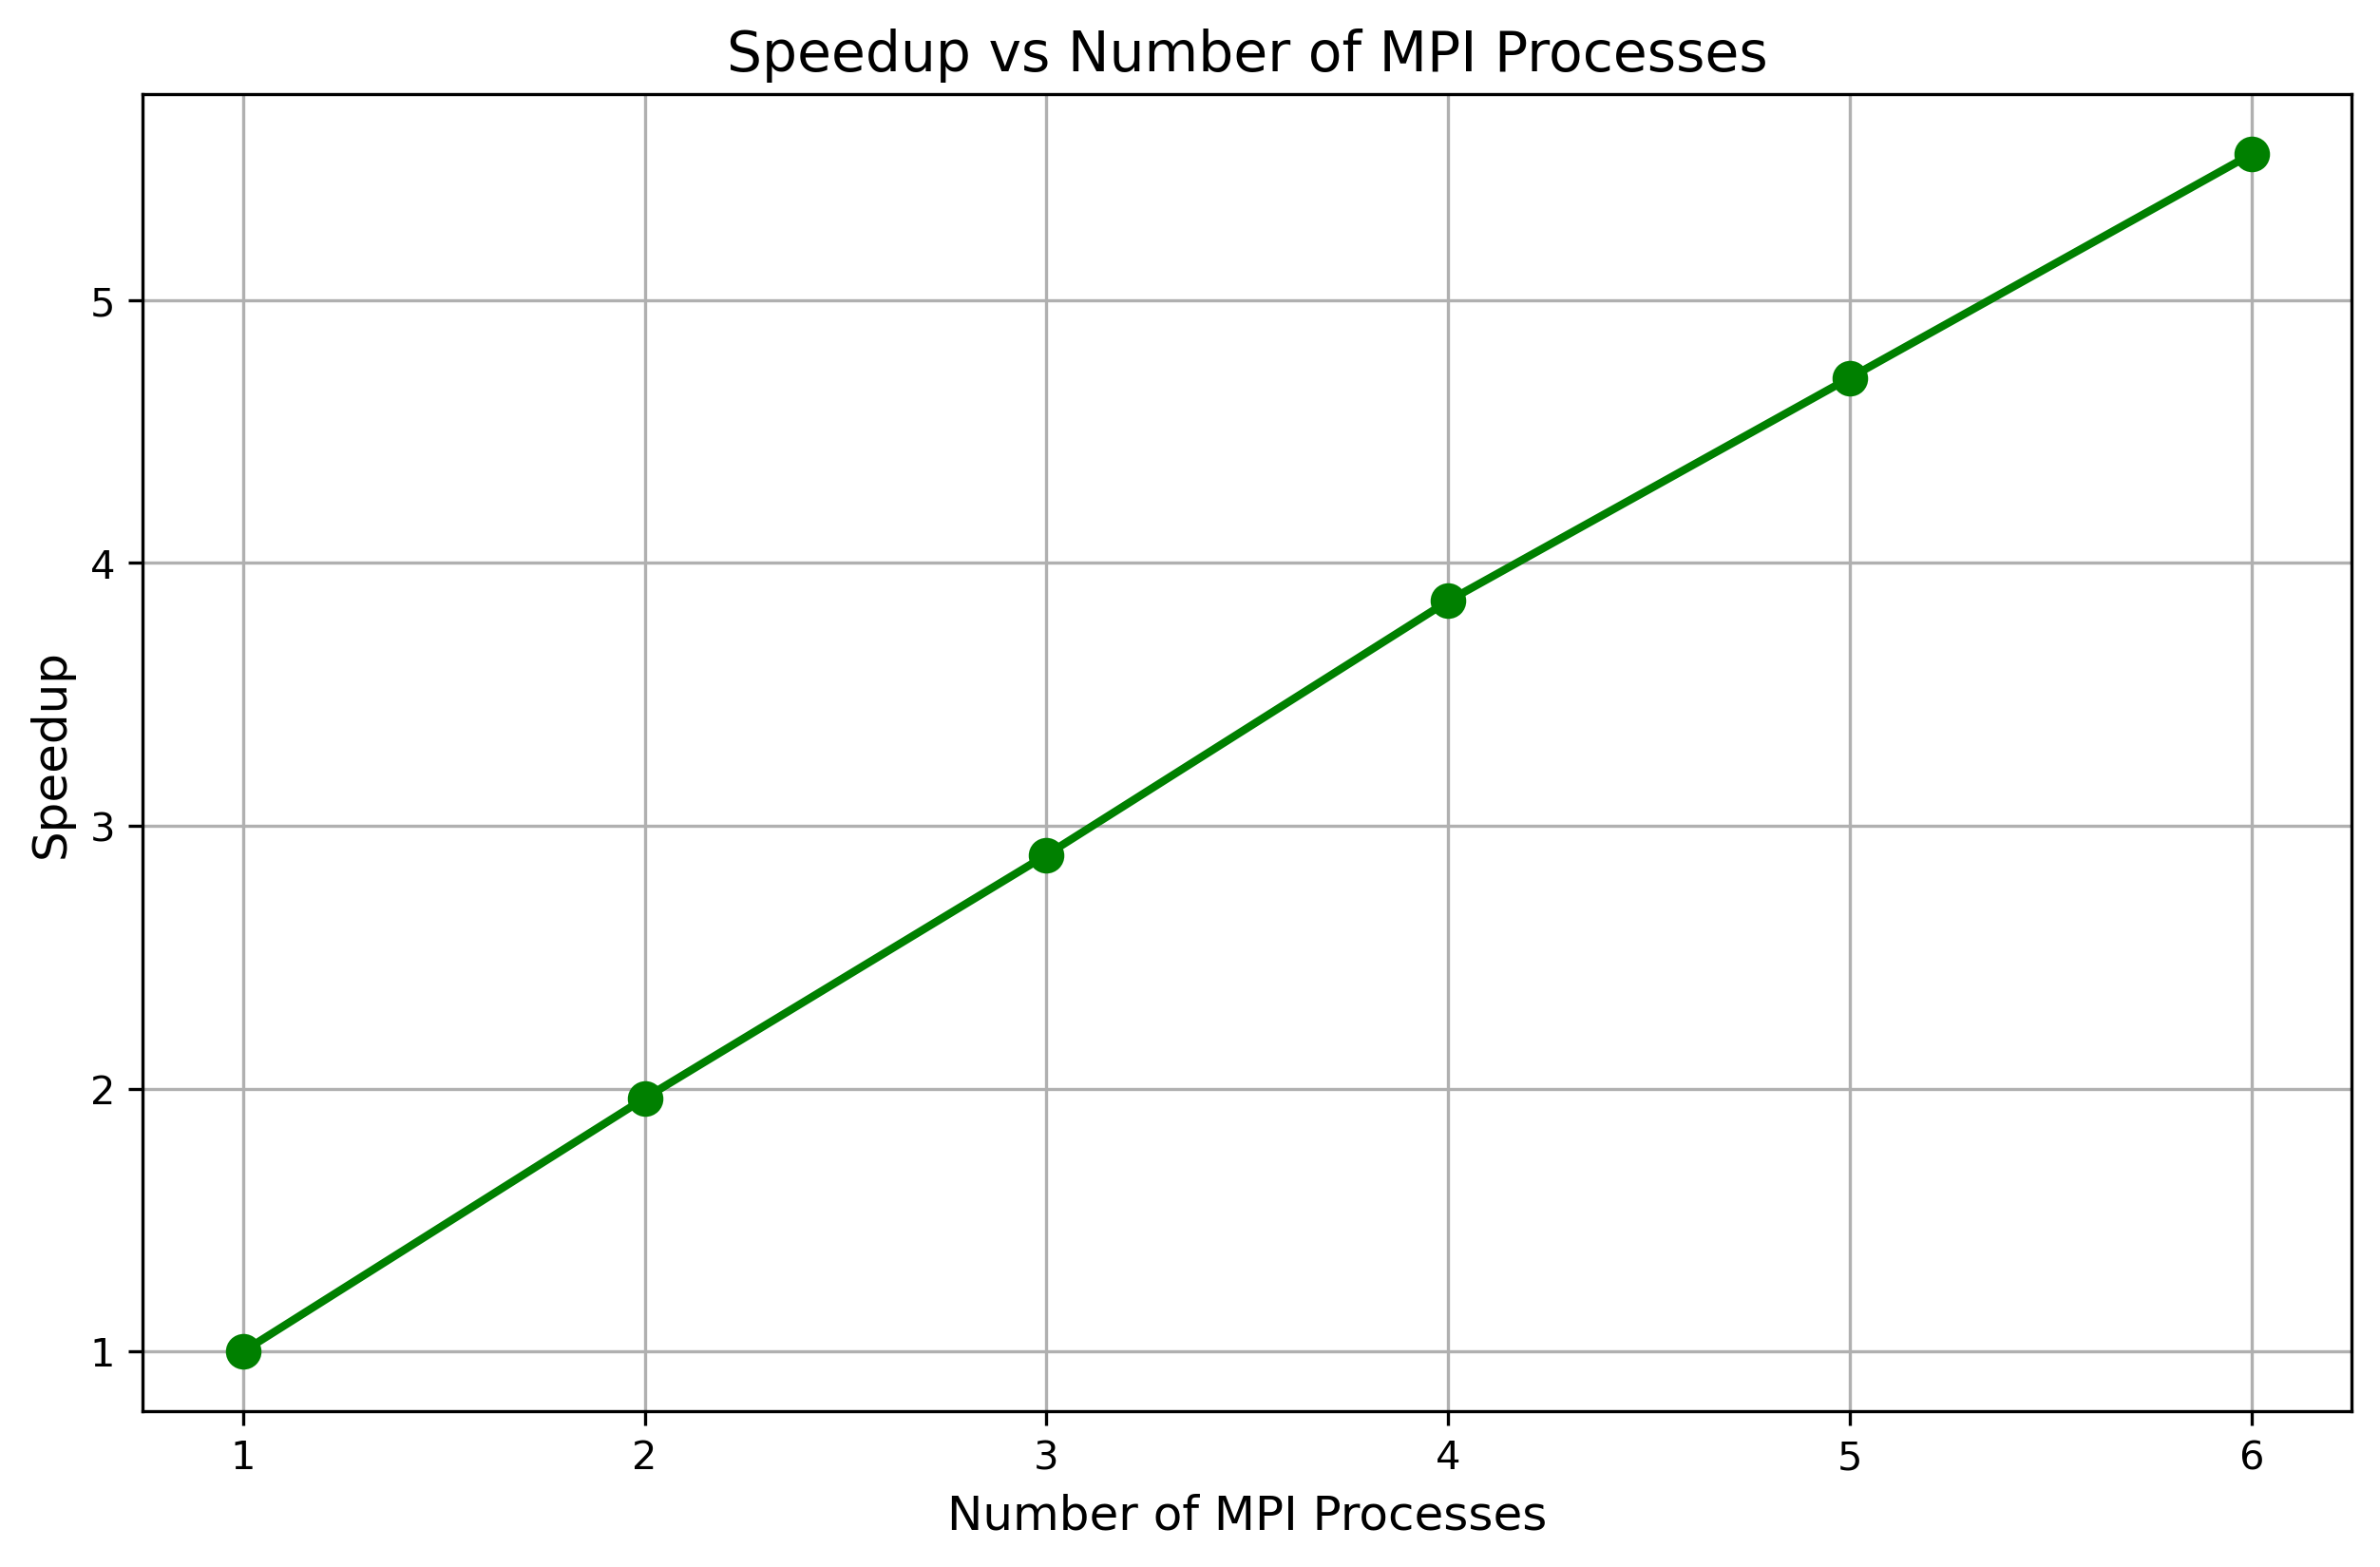
\includegraphics[width=0.8\textwidth]{speedup_vs_processes.png}
\caption{Speedup vs Number of MPI Processes}
\end{figure}

\section{Speedup Calculation}
The speedup is calculated using the formula:

\begin{equation}
\text{Speedup} = \frac{\text{Execution Time with 1 Process}}{\text{Execution Time with N Processes}}
\end{equation}

For example, with 6 processes:
\begin{align*}
\text{Speedup} &= \frac{198.77 \text{ seconds}}{35.78 \text{ seconds}} \\
&= 5.56
\end{align*}

\section{Efficiency Analysis}
The efficiency of the parallel implementation is calculated as:

\begin{equation}
\text{Efficiency} = \frac{\text{Speedup}}{\text{Number of Processes}} \times 100\%
\end{equation}

\begin{table}[H]
\centering
\begin{tabular}{|c|c|c|}
\hline
\textbf{MPI Processes} & \textbf{Speedup} & \textbf{Efficiency (\%)} \\
\hline
1 & 1.00 & 100.0 \\
2 & 1.96 & 98.2 \\
3 & 2.89 & 96.3 \\
4 & 3.86 & 96.4 \\
5 & 4.70 & 94.1 \\
6 & 5.56 & 92.6 \\
\hline
\end{tabular}
\caption{Speedup and efficiency for different numbers of MPI processes}
\end{table}

\section{Conclusion}
The parallel implementation of the mean shift clustering algorithm using MPI demonstrates significant performance improvements as the number of processes increases. With 6 processes, a speedup of 5.56 was achieved, which corresponds to an efficiency of 92.6\%. This indicates that the parallel implementation scales well with the number of processes, making it suitable for processing large datasets.

The slight decrease in efficiency as the number of processes increases can be attributed to communication overhead and load imbalance. However, the overall performance gain justifies the use of parallel processing for this application.

\end{document}
